%
% wege.tex
%
% (c) 2019 Prof Dr Andreas Müller, Hochschule Rapperswil
%
\begin{frame}
\frametitle{Wege statt Weglänge?}
\begin{columns}[t]
\begin{column}{0.48\hsize}
\begin{block}{Wege speichern?}
\uncover<3->{Es reicht, einen Wegweiser zum nächsten Knoten zu speichern}
\end{block}
\begin{center}
\begin{tikzpicture}[>=latex]

\end{tikzpicture}
\end{center}
\end{column}
\begin{column}{0.48\hsize}
\uncover<2->{%
\begin{center}
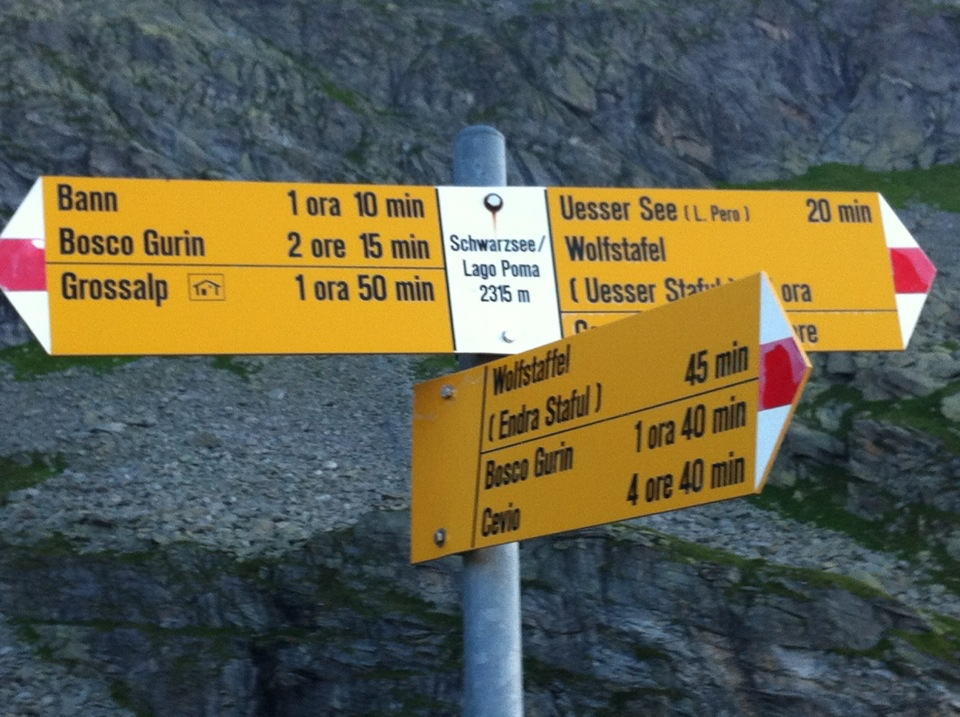
\includegraphics[width=\hsize]{../slides/8/floyd-warshall/wegweiser.jpg}
\end{center}}%
\end{column}
\end{columns}
\end{frame}
